\documentclass{article}

\usepackage[utf8]{inputenc}
\usepackage[catalan]{babel}
\usepackage{graphicx}
\usepackage{listings}
\usepackage{hyperref}

\graphicspath{{images/}}

\title{El Far}
\author{Kenan Rhoton}


\usepackage{color}

\definecolor{mygreen}{rgb}{0,0.6,0}
\definecolor{mygray}{rgb}{0.5,0.5,0.5}
\definecolor{mymauve}{rgb}{0.58,0,0.82}

\lstset{backgroundcolor=\color{white},   % choose the background color; you must add \usepackage{color} or \usepackage{xcolor}
  basicstyle=\footnotesize,        % the size of the fonts that are used for the code
  breakatwhitespace=false,         % sets if automatic breaks should only happen at whitespace
  breaklines=true,                 % sets automatic line breaking
  captionpos=b,                    % sets the caption-position to bottom
  commentstyle=\color{mygreen},    % comment style
  extendedchars=true,              % lets you use non-ASCII characters; for 8-bits encodings only, does not work with UTF-8
  frame=L,	                   % adds a frame around the code
  keepspaces=true,                 % keeps spaces in text, useful for keeping indentation of code (possibly needs columns=flexible)
  keywordstyle=\color{blue},       % keyword style
  language=Python,                 % the language of the code
  numbers=none,                    % where to put the line-numbers; possible values are (none, left, right)
  numbersep=5pt,                   % how far the line-numbers are from the code
  numberstyle=\tiny\color{mygray}, % the style that is used for the line-numbers
  rulecolor=\color{black},         % if not set, the frame-color may be changed on line-breaks within not-black text (e.g. comments (green here))
  showspaces=false,                % show spaces everywhere adding particular underscores; it overrides 'showstringspaces'
  showstringspaces=false,          % underline spaces within strings only
  showtabs=false,                  % show tabs within strings adding particular underscores
  stepnumber=1,                    % the step between two line-numbers. If it's 1, each line will be numbered
  stringstyle=\color{mymauve},     % string literal style
  tabsize=2,	                   % sets default tabsize to 2 spaces
}

\lstset{literate=
  {á}{{\'a}}1 {é}{{\'e}}1 {í}{{\'i}}1 {ó}{{\'o}}1 {ú}{{\'u}}1
  {Á}{{\'A}}1 {É}{{\'E}}1 {Í}{{\'I}}1 {Ó}{{\'O}}1 {Ú}{{\'U}}1
  {à}{{\`a}}1 {è}{{\`e}}1 {ì}{{\`i}}1 {ò}{{\`o}}1 {ù}{{\`u}}1
  {À}{{\`A}}1 {È}{{\'E}}1 {Ì}{{\`I}}1 {Ò}{{\`O}}1 {Ù}{{\`U}}1
  {ä}{{\"a}}1 {ë}{{\"e}}1 {ï}{{\"i}}1 {ö}{{\"o}}1 {ü}{{\"u}}1
  {Ä}{{\"A}}1 {Ë}{{\"E}}1 {Ï}{{\"I}}1 {Ö}{{\"O}}1 {Ü}{{\"U}}1
  {â}{{\^a}}1 {ê}{{\^e}}1 {î}{{\^i}}1 {ô}{{\^o}}1 {û}{{\^u}}1
  {Â}{{\^A}}1 {Ê}{{\^E}}1 {Î}{{\^I}}1 {Ô}{{\^O}}1 {Û}{{\^U}}1
  {œ}{{\oe}}1 {Œ}{{\OE}}1 {æ}{{\ae}}1 {Æ}{{\AE}}1 {ß}{{\ss}}1
  {ű}{{\H{u}}}1 {Ű}{{\H{U}}}1 {ő}{{\H{o}}}1 {Ő}{{\H{O}}}1
  {ç}{{\c c}}1 {Ç}{{\c C}}1 {ø}{{\o}}1 {å}{{\r a}}1 {Å}{{\r A}}1
  {€}{{\EUR}}1 {£}{{\pounds}}1 {™}{{\textsuperscript{TM}}}1
}

\begin{document}
\maketitle

\section{Presentació del projecte}

Amnistia Internacional és una organització no gubernamental que defensa els drets humans arreu del món. A Catalunya busquen prendre acció enfront de qualsevol llei o situació que violi aquests drets, i per a fer-ho han de gestionar moltíssima informació.

És aquí on entra aquest projecte: la cerca i ordenació de la informació.

Aquest projecte busca facilitar el màxim possible que qualsevol notícia d'interés per a Amnistia Internacional sigui inmediatament visible, indexada i accessible. Busca, en el fons, treure el màxim de feina a fer en quant a totes les accions que tenen a veure en la informació, per a que l'organització pugui centrar-se en prendre acció.

I és per això que aquest projecte, com un far, intenta ajudar l'usuari a no perdre's en un mar d'informació, sino tenir al seu abast tota la informació que necessita quan la necessita, automatitzant al màxim totes les cerques i peticions possibles.

\newpage

\tableofcontents

\newpage

\section{Objectius del projecte}

El objectiu principal d'aquest projecte es ser útil. El que prima per mi és que la eina desenvolupada compleixi completament la seva funció de facilitar les tasques de cerca d'informació que s'efectúen a Amnistia Internacional Catalunya.

Les tasques que es volen cobrir son:

\begin{description}
    \item[Detecció de notícies clau] Interessa poder saber cada dia quines notícies de la gran quantitat de fonts d'interés són realment rellevant per les causes que Amnistia Internacional defensa, sense haver de filtar la informació manualment
    \item[Indexació de la informació] Es vol que la informació quedi organitzada de manera que sigui fàcil filtrar-la i fer cerques, tant per data, com per contigut, temàtica y font.
    \item[Extensibilitat] És important que el sistema es pugui extendre fàcilment, que hi hagi un métode senzill que permeti afegir noves fonts d'informació i idealment que sigui fàcil que algú que no conegui el sistema pugui afegir-hi funcionalitats.
    \item[Flexible] El sistema ha de funcionar per fonts de diferents tipus, ja siguin pàgines web com documents amb actualitzacions periòdiques (PDF, DOC, etc.), y ha de ser fàcil canviar els paràmetres de cerca, ja que els temes d'interés varien en el temps.
    \item[Usabilitat] El sistema ha de ser senzill i intuitiu, sense requerir uns alts coneixements tècnics pel seu correcte funcionament.
    \item[Obert] Finalment, un objectiu personal és que el sistema no només sigui útil per a Amnistia, sinó que, sense cap detriment al funcionament necessitat per ells, pugui tenir múltiples utilitats i pugui potencialment ser utilitzat per tothom que necessiti qualsevol sistema similar.
\end{description}

\newpage

\section{Planificació inicial}

En primer lloc es farà un estudi de l'estat de l'art i un anàlisi dels requisits del sistema. Seguidament es seguira una metodologia àgil amb sprints de dues setmanes.

En els sprints de dues setmanes s'inclourà:

\begin{description}
    \item[Evolució dels requisits] És important, amb fi d'assegurar que entenem bé el problema del client, adaptar els requisits sobre qué ha d'oferir el sistema.
    \item[Disseny] També cal establir el funcionament general del sistema i tenir clar com es resoldràn cadascun dels problemes s'intenten solucionar amb el sistema.
    \item[Implementació] El sistema s'ha de construir de manera que puguem adaptar-lo en cas de que sigui necessària qualsevol modificació, intentant que tingui la major modularitat possible.
    \item[Verificació] Finalment, cal comprobar el correcte funcionament del sistema tant a nivell técnic com a nivell de compliment de requisits i assoliment d'objectius.
\end{description}

Es calcula que seràn necessaris sis sprints, amb una dedicació d'unes 20 hores per sprint.

Per assegurar que el sistema en tot moment estigui en un estat en que cadascun dels punts és verificable (és a dir, que es pot comprovar quins objectius i requisits ja s'han complert i que respecten les decisions de disseny) es farà servir una metodologia del tipus \emph{test-driven} per garantir en la major mesura possible que s'estàn assolint les funcionalitats que cerquem.

També es farà una documentació constant de tot el procés i de totes les comprovacions que es fan, així com totes les funcionalitats que es desenvolupen.

Finalment, quan s'hagin assolit els objectius, es farà una passada final que comprovi en profunditat la capacitat d'us del sistema en conjunt amb Amnistia Internacional, i es farà una valoració de tot el treball.

\newpage

\section{Estat de l'art}

El primer pas, com en qualsevol projecte, ha sigut investigar les solucions ja existents i si s'adequen o no com a solució al problema que té Amnistia Internacional.

\subsection{Google}

La primera eina que ve al cap al pensar en el problema és, evidentment, Google.

Si bé és veritat que una cerca a Google fent servir limitacions per pàgina web, paraules clau i data donaria alguns resultats, no es trobarien tots ja que depén també de la implementació de l'algorisme de Google per determina qué ``és interessant''.

Adicionalment, esdevindria complicat gestionar tot el tema de les paraules clau degut a que requeriría fer servir una tira enorme de paraules i frases amb conectors, cosa que no és ni pràctica ni escalable ni usable, i per tant pot acabar sent més una font d'errors i de pérdues de temps que no pas una manera de solucionar el problema que pretén solucionar Amnistia Internacional.

\subsection{Versionista}

Versionista es la primera eina més ``seria'' que trobem al buscar alguna manera de seguir els canvis realitzats a una web. Funciona de una manera extremadament senzilla: a través de les URLs que volem monitoritzar, senzillament detecta quins canvis s'han produït cada dia.

Lamentablament, no ens permet filar més prim que això, i corre a càrrec de l'usuari el distingir quins canvis són rellevants i quins no, i per tant falla en un aspecte crucial: no ens permet filtrar les novetats segons els nostres interessos.


\subsection{VisualPing}

Aquesta eina, tot i que va començar com una alternativa a Versionista, té considerablement més problemes, ja que no només no pot distingir zones de una plana web, sino que tampoc pot distingir anuncis, i per tant qualsevol web que tingui algún tipus de publicitat canviant donará molts falsos positius.

\subsection{Google Docs}

Una opció molt curiosa que existeix és la de crear un arxiu de Google Docs i mitjançant la eina ImportXML especificar amb XPath parts de webs que volem controlar.

Tot i ser una opció prou precisa, requereix un altíssim nivell tècnic per gestionar i te la gran desavantatge de que no es capaç de processar documents PDF o Word, requisit indispensable per a Amnistia Internacional.

\subsection{WebSite-Watcher}

Una de les primeres eines en crearse, lamentablement no és gratuïta, és de codi tancat i no permet filtrar en profunditat els resultats, pel qual va quedar immediatament descartada.

\subsection{Distill Web Monitor}

Aquesta extensió de Firefox té casi totes les funcionalitats que busquem: permet definir seccions de pàgines web i filtrar per paraules clau (a través d'expressions regulars, per això).

Però, com totes les altres eines, té un problema crític: No ens dona la opció de processar els documents trobats.

\subsection{Conclusió}

Tot i que n'hi han unes quantes eines que s'apropen més o menys al que es busca, cap realment és una solució completa que permeti cercar i indexar la informació trobada a documents PDF\".

\newpage

\section{Anàlisi del problema}

Tot projecte comença a partir d'un problema que es pretén solucionar. En aquesta secció detallem en profunditat el problema que te Amnistia Internacional de Catalunya abans del començament d'aquest projecte.

\subsection{Eficiència del temps}

En primer lloc, el problema que té AIC és un problema de temps. Es perd molt de temps mirant notícies individuals a moltes fonts diferents per decidir si són o no d'interés. Aquestes fons sont molt diverses i no segueixen un mateix patró estructural: de fet, algunes fonts son pàgines web i d'altres són documents PDF\@.

Ja inicalment podem intuir que algún tipus de software pot ajudar a resoldre aquest problema, fent servir algún tipus de cerca i indexació de la informació per automatitzar la tasca repetitiva. Però també ja s'intueix algún problema a la falta d'estructura comuna de les diferents fonts: potser saber on buscar la informació no és trivial\ldots

\subsection{Error humà}

Degut a la gran quantitat de fonts i paraules clau, és bastant probable que al fer-ho manualment hi hagin notícies d'importància per a Amnistia Internacional de Catalunya que no es vegin a primer cop d'ull, cosa que fa que a més de ser una tasca bastant pesada, no sigui del tot acurada.

Un sistema informàtic, per definició, eliminaria aquest error, fent que la quantitat de notícies que passen desapercebudes sigui molt menor (idealment zero).

\subsection{Indexació}

Finalment, els hi seria molt pràctic poder consultar notícies anteriors d'interès sense haver de guardar-les manualment, sigui per data o paraules clau.

Clar està que les bases de dades ens ajudaríen infinitament en aquest aspecte!

\newpage

\section{Solució inicial}

\subsection{Model de Dades}

Com a solució inicial es va plantejar un sistema amb els següents elements de la base de dades:

\begin{description}
        \item[Fonts] Adreces web on es busca la informació que volem. Contenen una URL on es cerca la informació i un XPath que indica la posició exacta de la web on apareixen les notícies.
        \item[Catàlegs] Conjunts de paraules clau que indiquen qué és d'interés per a nosaltres.
        \item[Notícies] Coincidencies trobades amb les Paraules Clau esmentades dins les Fonts.
\end{description}

Aquests elements es relacionen de la següent manera:

\begin{figure}[!ht]
    \centering
    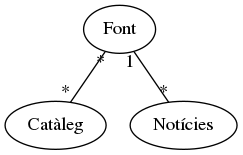
\includegraphics[scale=1]{db.png}
    \caption{Model de Dades}
\end{figure}

\newpage

A continuació adjuntem el codi dels models comentat:

\begin{lstlisting}
# Aquest model conté informació sobre les Font's d'informació.
# -   nom: conté el nom donat per l'administrador a la font
# -   url: conté la adreça web de la font
# -   webfile: conté el contingut de la font a la última actualització
# -   horari: conté la hora del servidor en la que s'actualitzará la font
class Font(models.Model):
    nom = models.CharField(max_length=200)
    url = models.URLField(max_length=200)
    webfile = models.FileField(upload_to='filtre.WebFileModel/dades/nom/mimetype', blank=True, null=True)
    horari = models.TimeField('Hora d\'actualització')
    catalegs = models.ManyToManyField('Cataleg', blank=True)
    def __str__(self):
        return self.nom

    def save(self, *args, **kwargs):
        delete_file_if_needed(self, `webfile')
        super(Font, self).save(*args, **kwargs)

    def delete(self, *args, **kwargs):
        super(Font, self).delete(*args, **kwargs)
        delete_file(self, `webfile')

# Aquest model conté informació sobre els Catàlegs de paraules d'interés
# -   nom: conté el nom donat per l'administrador al Catàleg
# -   frases: conté les frases que conformen el Catàleg
# -   fonts: conté les asociacions a les Fonts que fan servir el Catàleg
class Cataleg(models.Model):
    nom = models.CharField(max_length=200)
    frases = models.TextField()
    fonts = models.ManyToManyField(Font, blank=True)
    def __str__(self):
        return self.nom

# Aquest model conté informació sobre els Avisos
# -   coincidencia: Part del document que ha fet saltar l'Avís
# -   tipus: Indica si l'Avís ha saltat en un Document o a una Web
# -   pagina: En cas de ser tipus Document, conté la pàgina que ha provocat l'Avís
# -   url: adreça electrónica on hi ha el document o web
# -   data: conté la data en que va saltar l'Avís
# -   font: conté la font on va saltar l'Avís
class Avis(models.Model):
    coincidencia = models.CharField(max_length=2000)
    tipus = models.CharField(max_length=20) #Pot ser Document o Web
    pagina = models.IntegerField(null=True)
    url = models.URLField(max_length=2000) #Potencialment no és el mateix que el de la Font (si es d'un document intern)
    data = models.DateTimeField("Data de l'avís", null=True, blank=True)
    font = models.ForeignKey(Font)
    def __str__(self):
        return self.coincidencia
    class Meta:
        verbose_name = "avís"
        verbose_name_plural = "avisos"

## FOR DB FILE STORAGE

# Aquest model conté informació sobre els Arxius de contingut de les Fonts (ja que Heroku no ens dona llibertat amb el disc dur)
# -   dades: conté les dades en format Unicode
# -   nom: nom de l'arxiu
# -   mimetype: tipus MIME de l'arxiu
class WebFileModel(models.Model):
    dades = models.TextField()
    nom = models.CharField(max_length=255)
    mimetype = models.CharField(max_length=50)
\end{lstlisting}


\newpage

\subsection{Casos d'us}



\subsubsection{Afegir una font}

\begin{description}
    \item[Escenari]: Un usuari vol afegir una font
    \begin{description}
        \item[Donat] que som a la pàgina d'administració
        \item[Quan] l'usuari s'autentica correctament com a administrador
        \item[I] fa clic a la secció ``Fonts''
        \item[I] fa clic a ``Afegir font''
        \item[I] omple els camps amb nom, url, horari d'actualització i, opcionalment, els catàlegs rellevants
        \item[I] guarda la font
        \item[Aleshores] al visitar la pàgina principal apareix la font creada al llistat de fonts
    \end{description}
\end{description}

\subsubsection{Afegir un catàleg}

\begin{description}
    \item[Escenari]: Un usuari vol afegir un catàleg
    \begin{description}
        \item[Donat] que som a la pàgina d'administració
        \item[Quan] l'usuari s'autentica correctament com a administrador
        \item[I] fa clic a la secció ``Catàlegs''
        \item[I] fa clic a ``Afegir catàleg''
        \item[I] omple els camps amb nom, paraules clau i, opcionalment, les fonts on es fa servir
        \item[I] guarda el catàleg
        \item[I] visita la pàgina principal
        \item[I] fer clic en una font que estigui relacionada amb el catàleg
        \item[Aleshores] apareix el catàleg a la llista de catàlegs de la font
    \end{description}
\end{description}

\subsubsection{Consultar els avisos}

\begin{description}
    \item[Escenari]: Un usuari vol consultar els avisos recents
    \begin{description}
        \item[Donat] que som a la pàgina principal
        \item[I] que existeix algún avís recent
        \item[Aleshores] apareix el llistat de avisos recents
    \end{description}
\end{description}

\subsubsection{Consultar una font}

\begin{description}
    \item[Escenari]: Un usuari vol consultar els avisos recents d'una font específica
    \begin{description}
        \item[Donat] que som a la pàgina principal
        \item[I] que existeix algún avís recent de la font
        \item[Quan] l'usuari clica sobre la font que vol comprovar
        \item[Aleshores] apareixen els detalls de la font
        \item[I] el llistat de avisos recents d'aquella font
    \end{description}
\end{description}

\subsubsection{Consultar la informació d'un avís}

\begin{description}
    \item[Escenari]: Un usuari vol consultar la informació d'un avís
    \begin{description}
        \item[Donat] que som a la pàgina principal
        \item[I] que existeix algún avís recent
        \item[Quan] l'usuari clica sobre l'avís que vol comprovar
        \item[Aleshores] apareixen els detalls de l'avís
        \item[I] l'usuari pot clicar a l'enllaç proporcionat per veure l'avís sencer a la font original
    \end{description}
\end{description}


\newpage

\subsection{Vistes}

Com a solució inicial es va optar per una aplicació dividida en dues vistes: configuració i resultats.

La vista de configuració és un panell d'administració en el qual es poden afegir, eliminar i modificar les Fonts, Notícies i Avisos. És una vista senzilla amb l'objectiu de poder introduïr les dades necessàries per poder fer servir el sistema: Url y XPath de les Fonts i els Catàlegs de paraules.

A continuació tenim captures de pantalla de les vistes del panell d'administració:

\begin{figure}[!ht]
    \centering
    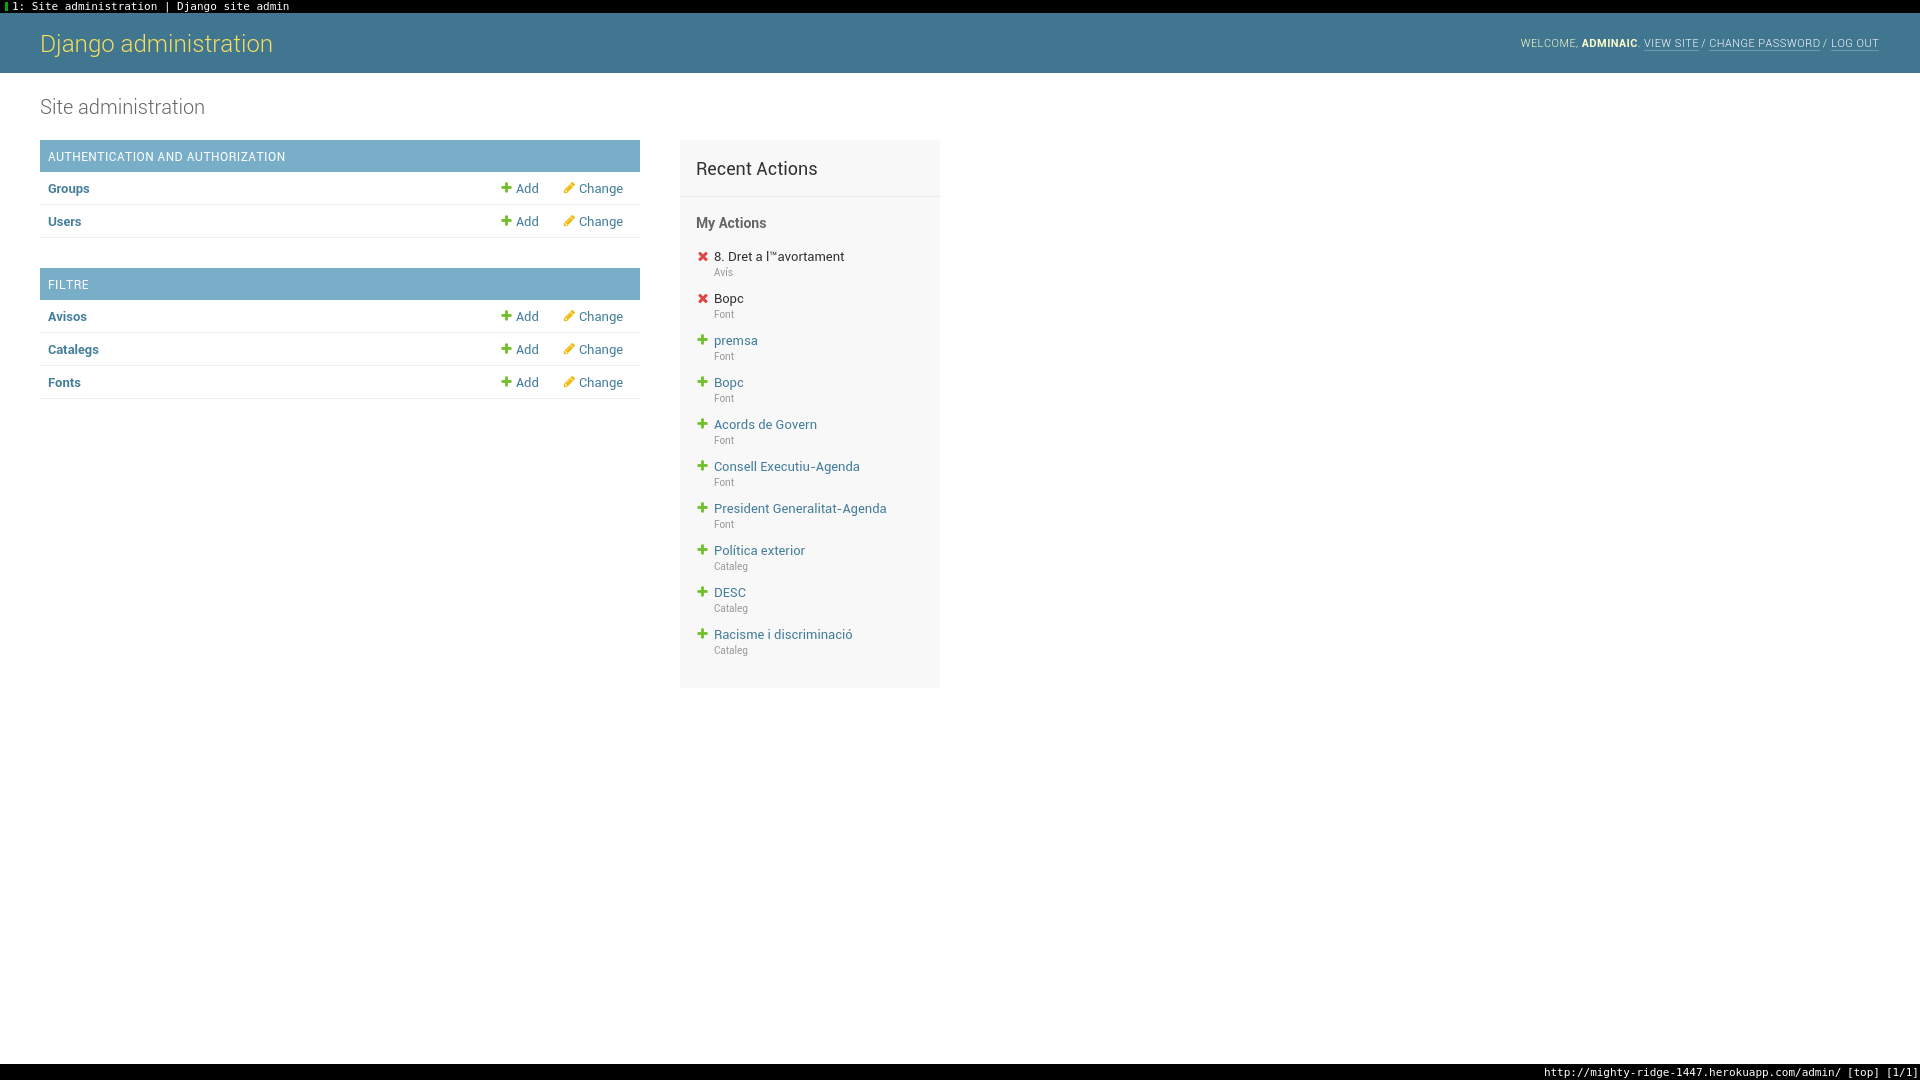
\includegraphics[width=0.8\textwidth]{adminpanel.png}
    \caption{Panell d'administració}
\end{figure}

\begin{figure}[!ht]
    \centering
    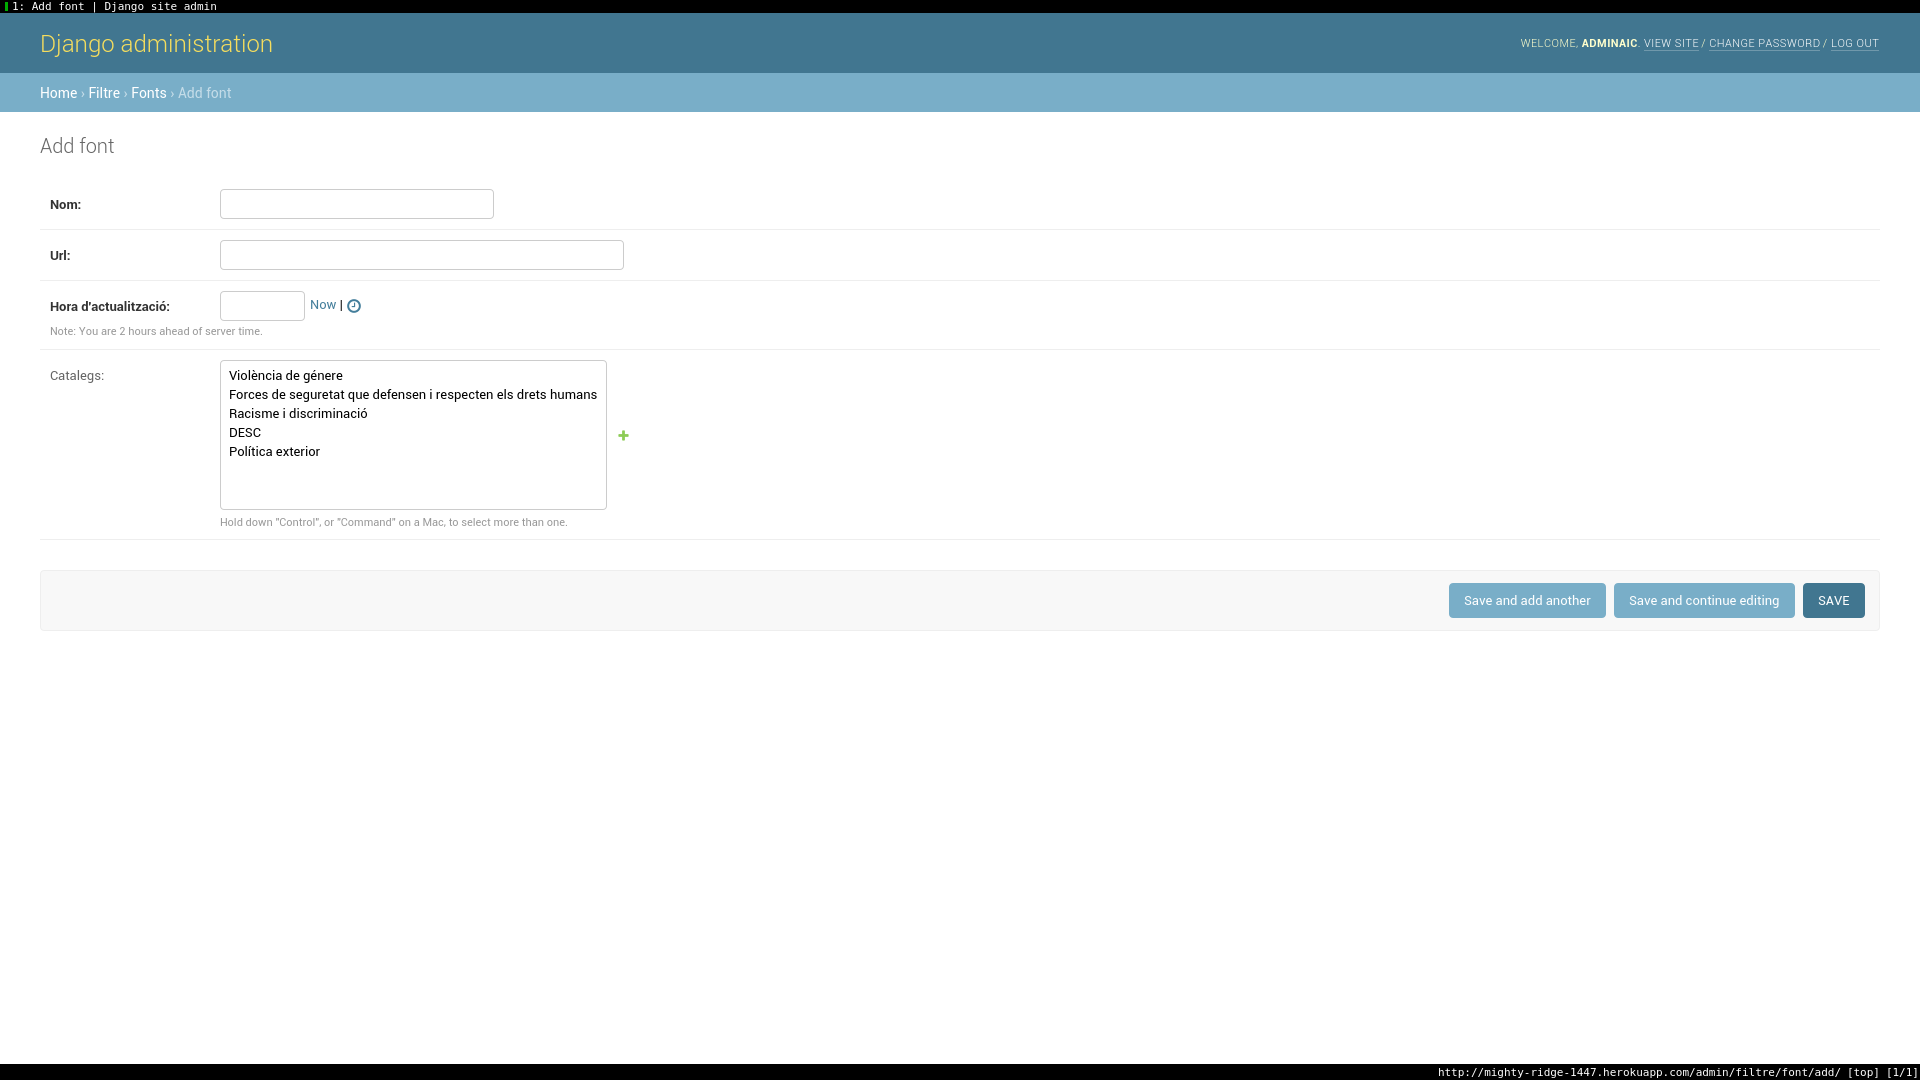
\includegraphics[width=0.8\textwidth]{addfont.png}
    \caption{Vista de Font}
\end{figure}

\newpage

\begin{figure}[!ht]
    \centering
    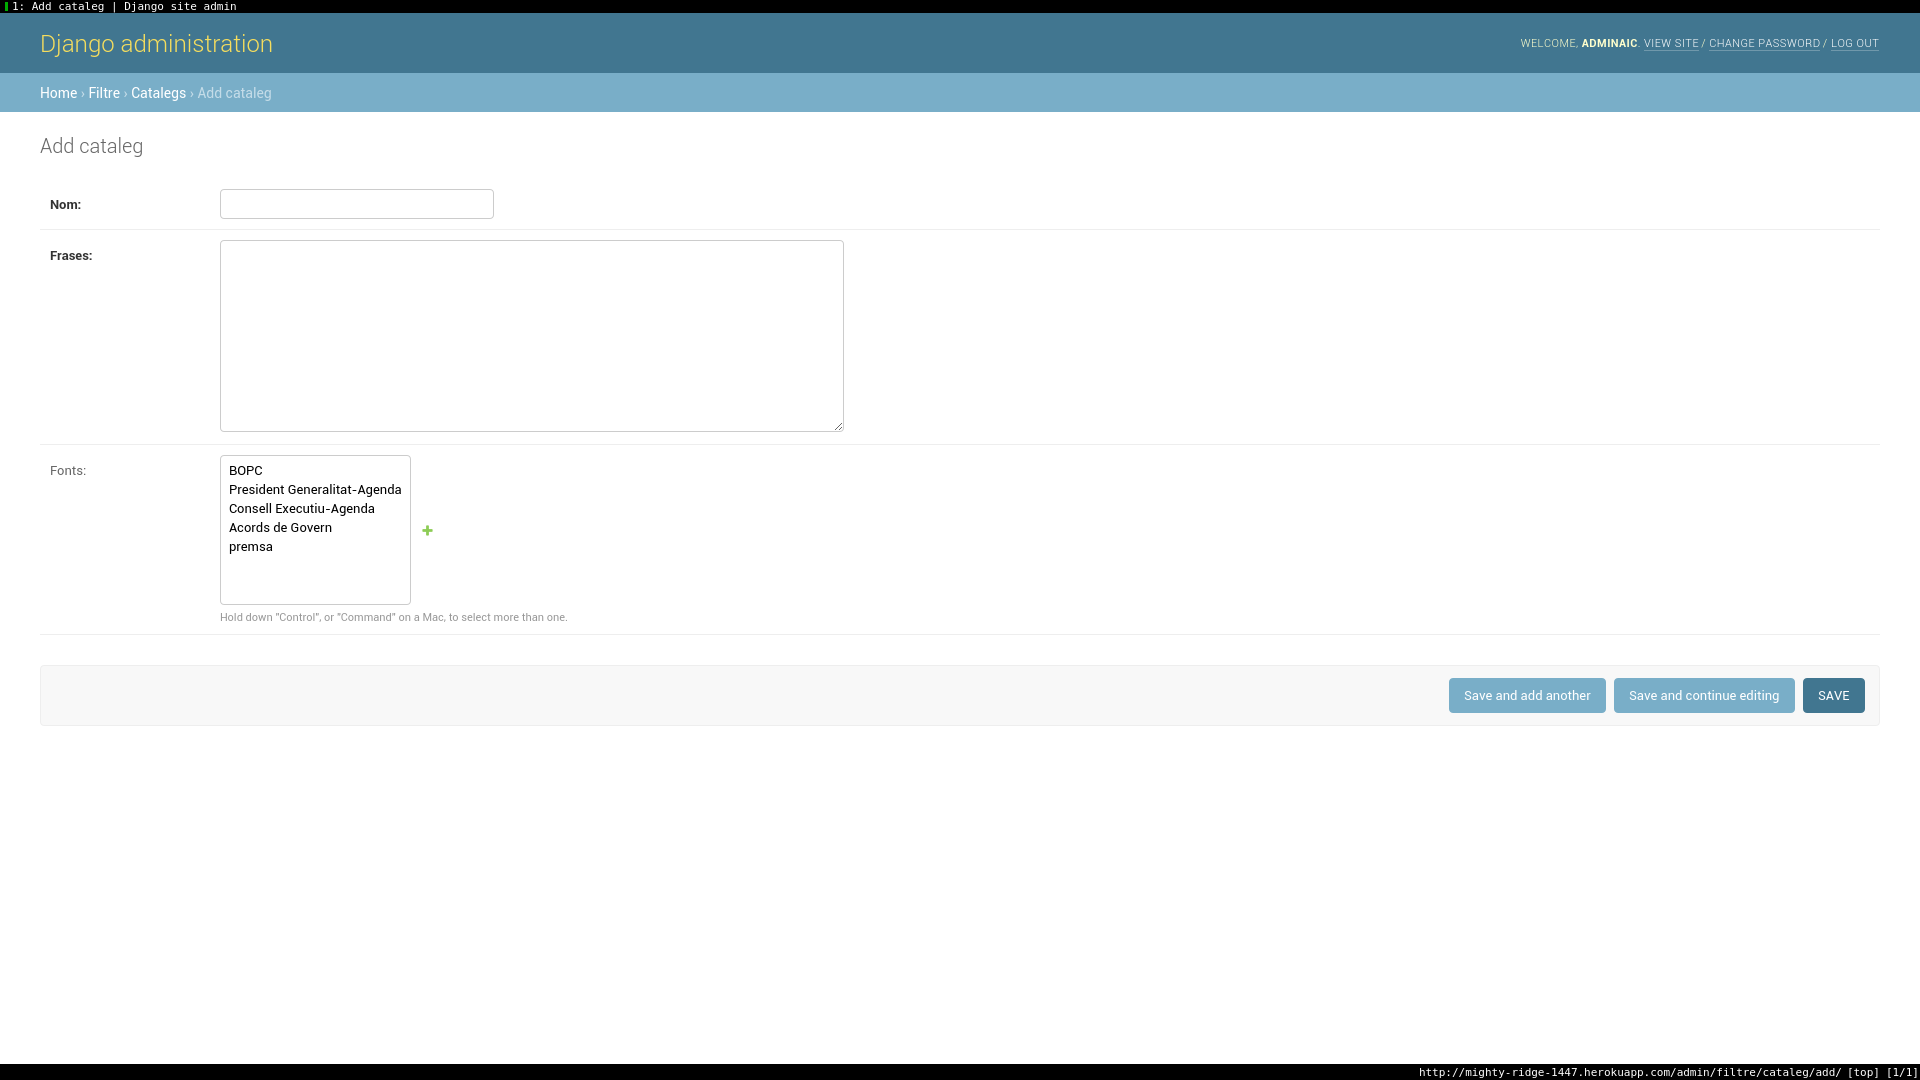
\includegraphics[width=0.8\textwidth]{addcataleg.png}
    \caption{Vista de Catàleg}
\end{figure}

\begin{figure}[!ht]
    \centering
    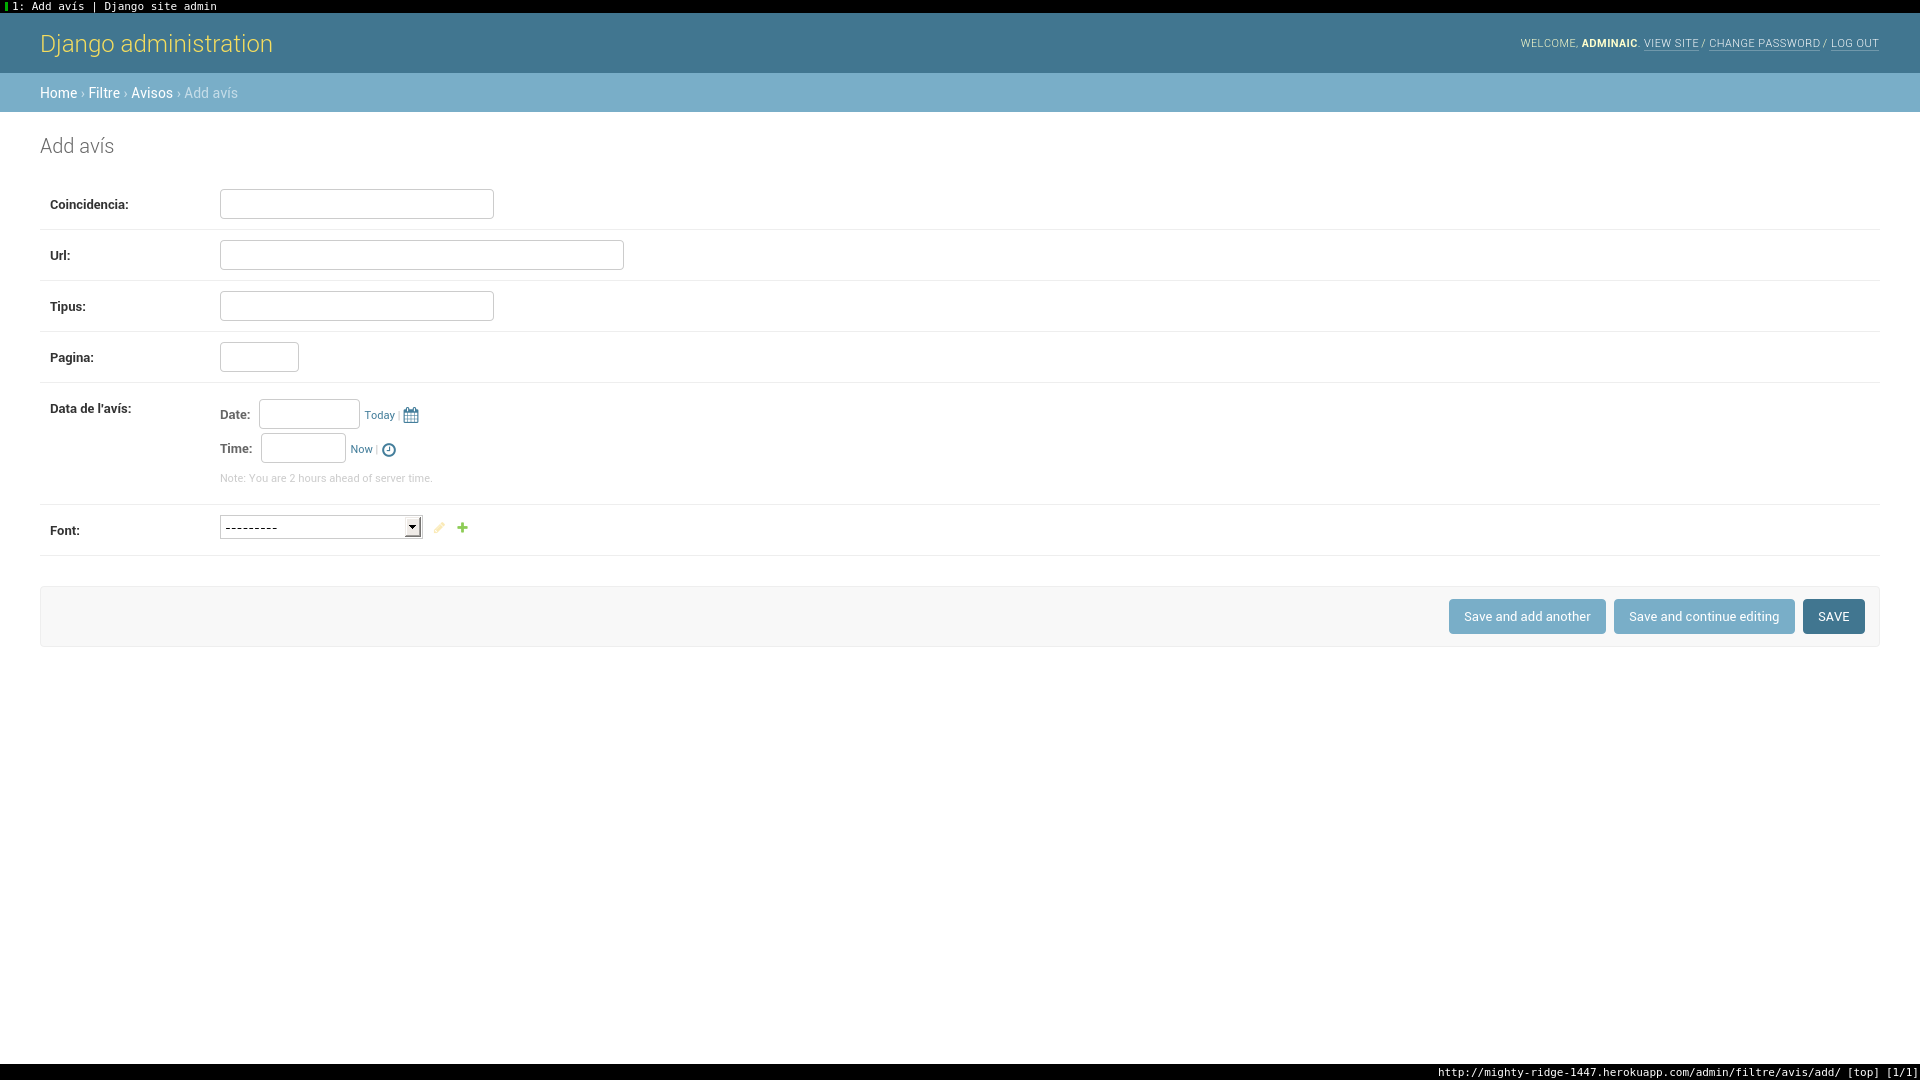
\includegraphics[width=0.8\textwidth]{addavis.png}
    \caption{Vista de Notícia}
\end{figure}

\newpage

Com veiem a més dels paràmetres bàsics hi han altres com l'hora d'actualització de la font, que és el moment del dia en el qual es comprovarà si hi han notícies de la Font en qüestió.

L'altra vista és la de resultats, que es divideix entre el resum de resultats, el detall d'una font i el detall d'una notícia.


\begin{figure}[!ht]
    \centering
    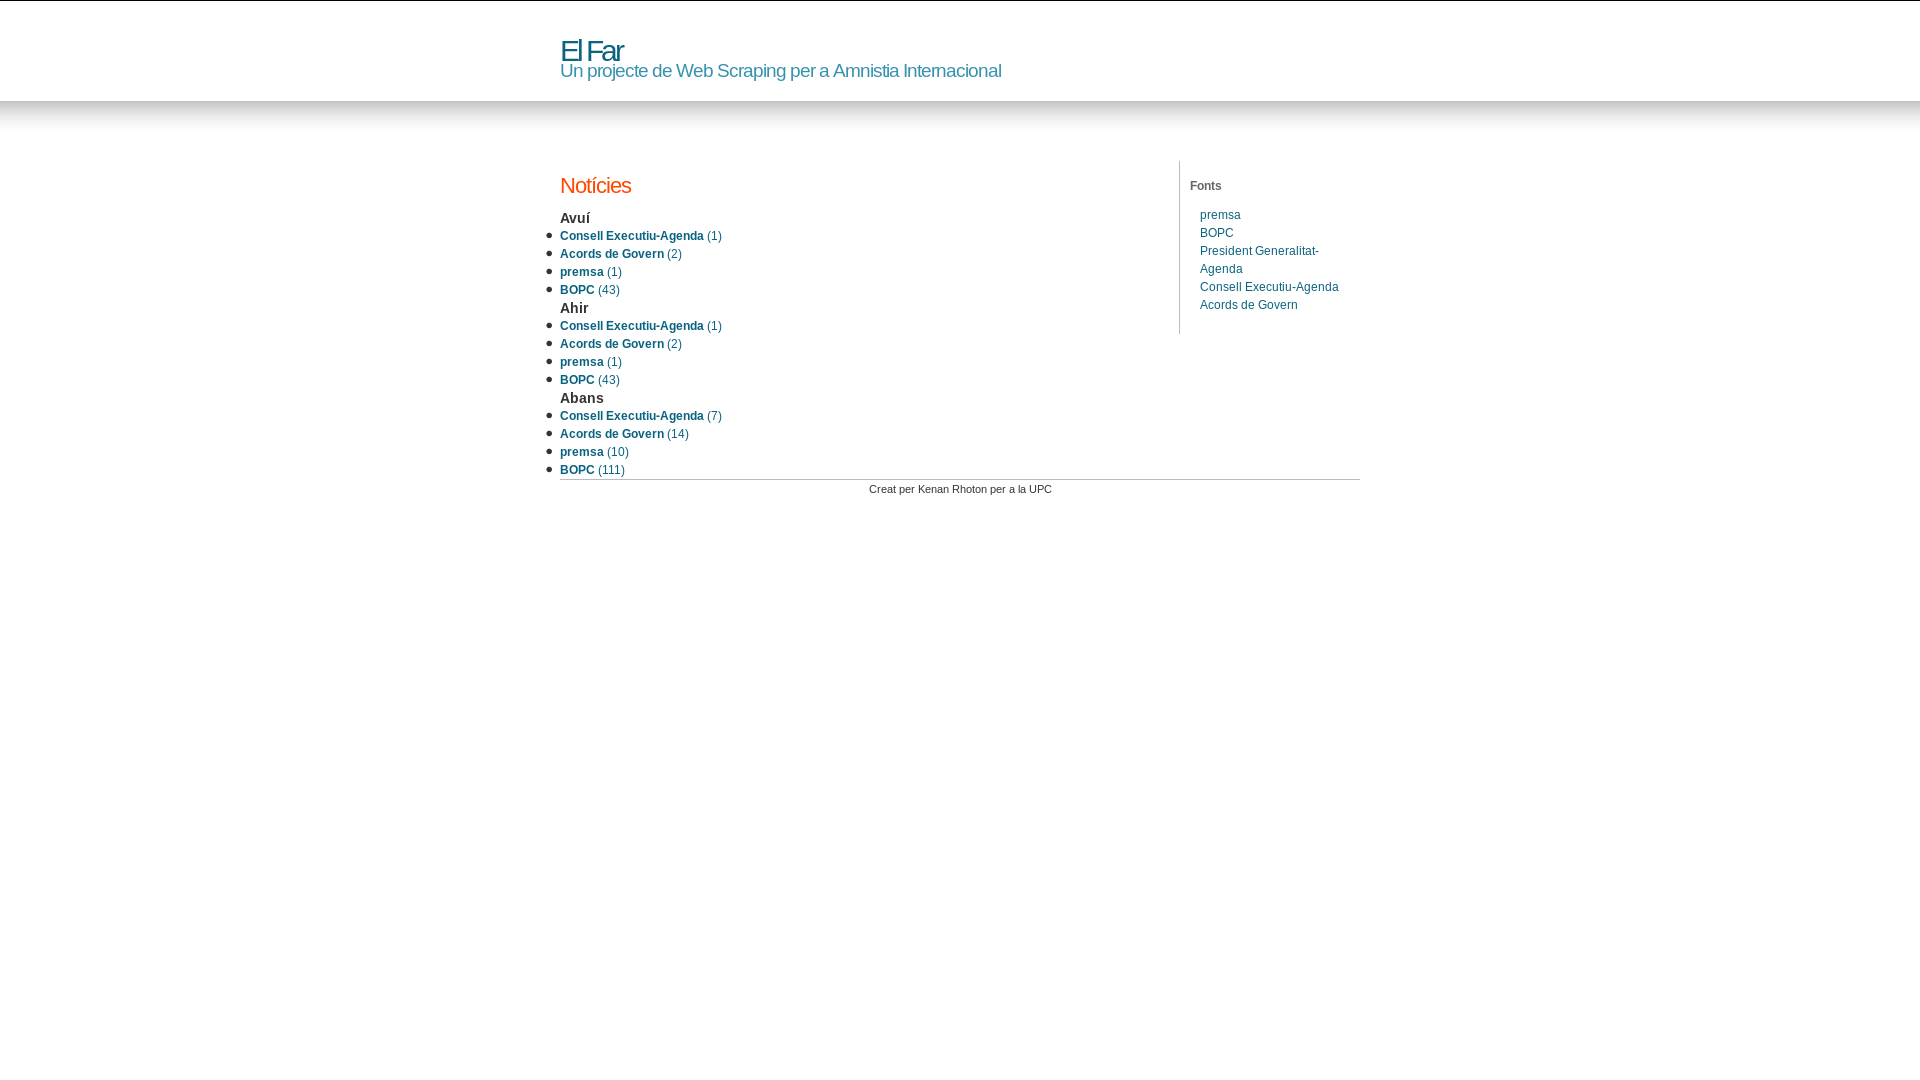
\includegraphics[width=0.8\textwidth]{resum.png}
    \caption{Resum de notícies}
\end{figure}

\begin{figure}[!ht]
    \centering
    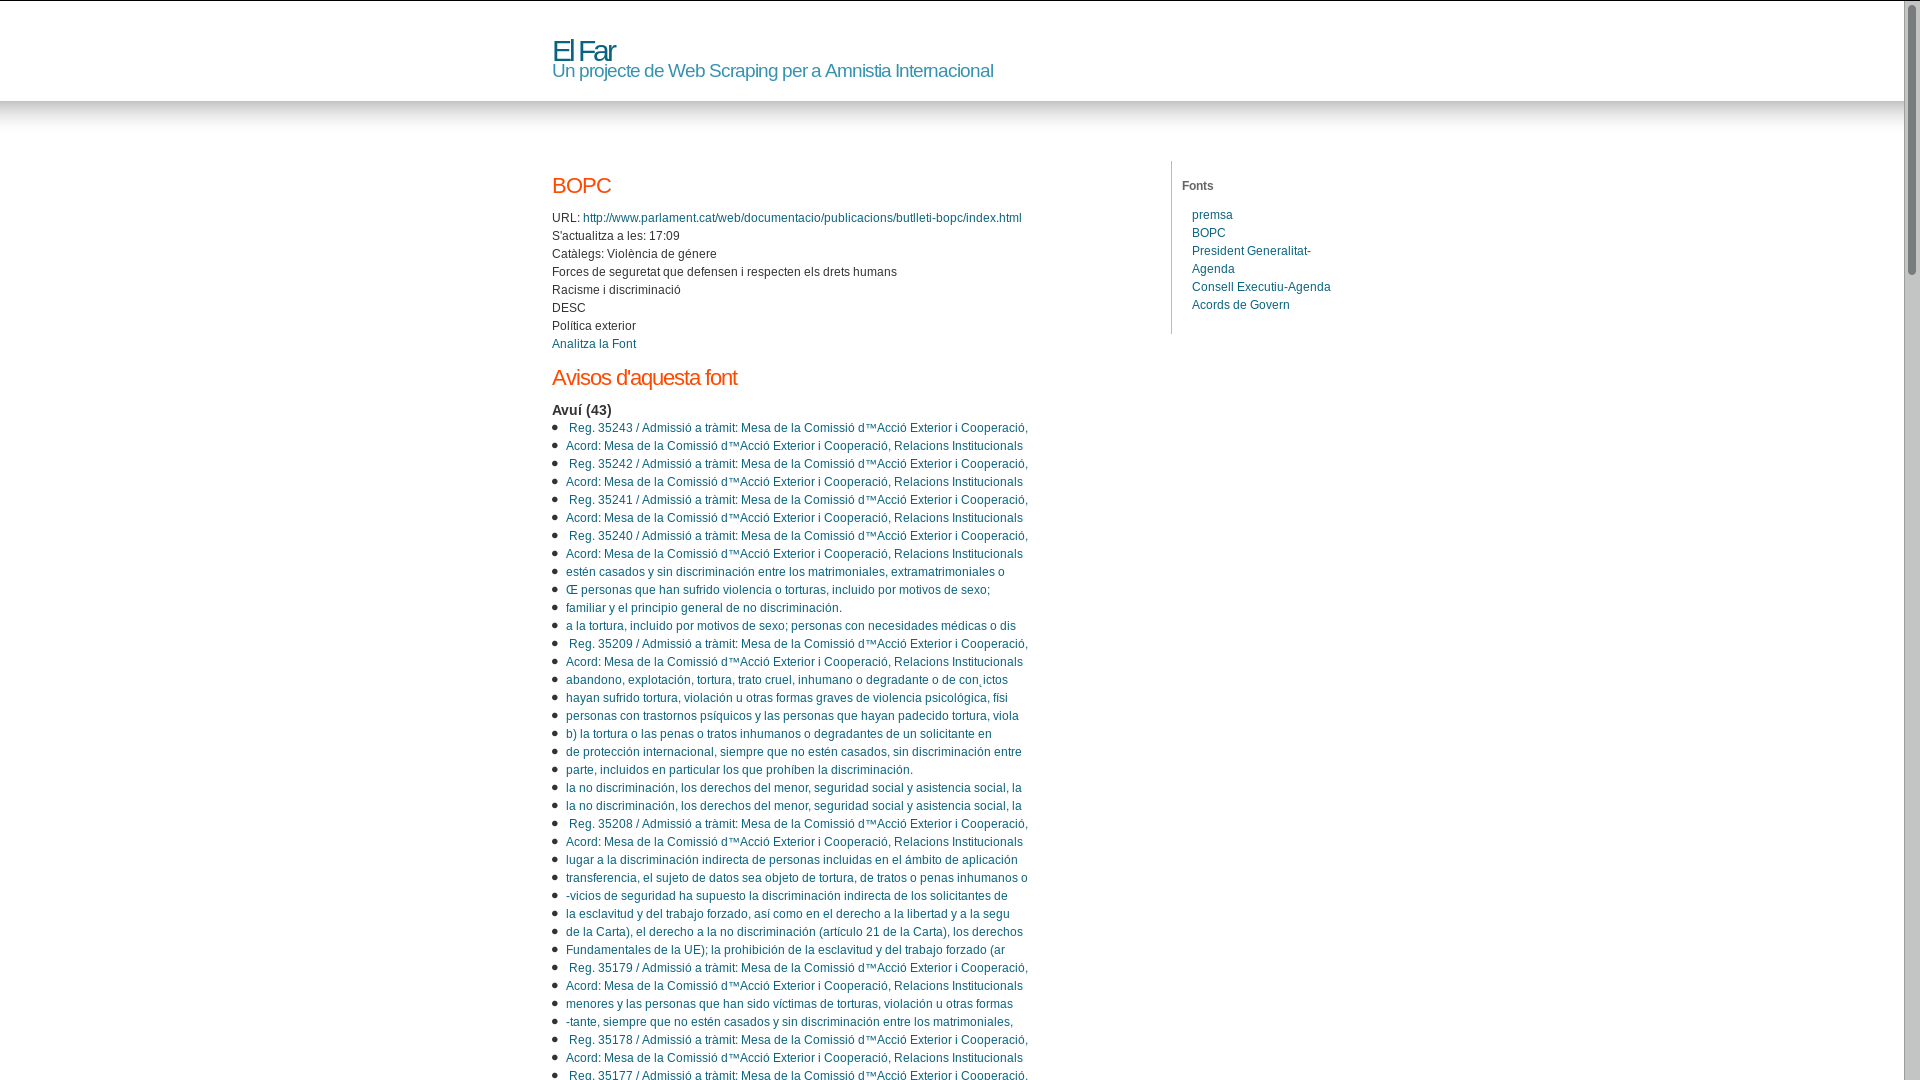
\includegraphics[width=0.8\textwidth]{detall_font.png}
    \caption{Detall Font}
\end{figure}

\newpage

\begin{figure}[!ht]
    \centering
    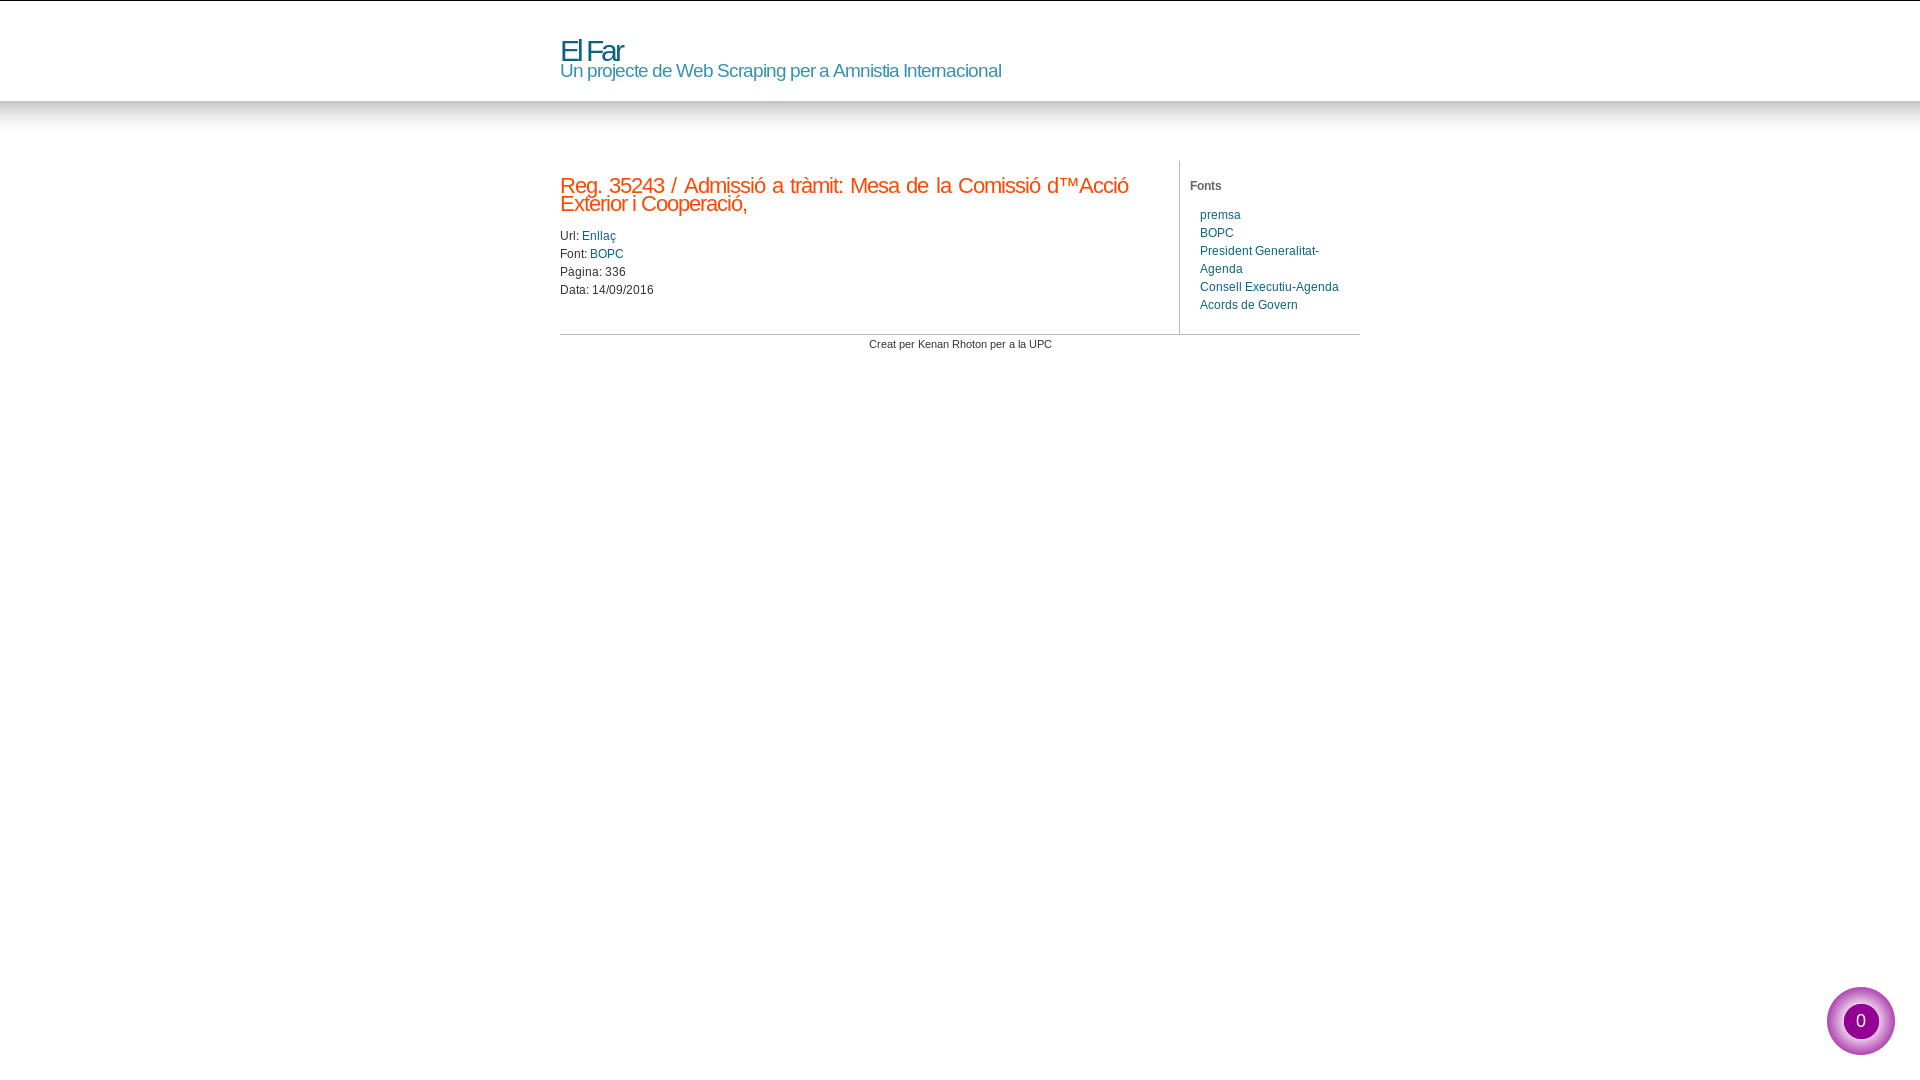
\includegraphics[width=0.8\textwidth]{detall_avis.png}
    \caption{Detall Avís}
\end{figure}

\newpage

\subsection{Funcionament}

El funcionament de la plataforma es pot dividir en 3 parts: BD, sistema Django i workers.

La BD es un PostgreSQL configurat per funcionar amb Heroku i Django sense cap misteri, i res del codi tracta directament amb ella: tot es fa a través dels models de Django. Tot i això, compleix la important funció de guardar tota la informació de les Fonts, Catàlegs i, sobretot, Notícies per poder fer-hi cerques amb bona velocitat.

El sistema Django fa tant la interfície amb l'usuari com la part funcional. La interfície está disenyada amb el sistema de plantilles de Django, que permet incorporar dades de dins l'aplicació Django en arxius HTML\@. La part funcional explota tot l'aspecte Python de Django al gestionar totes les peticions.

Ara bé, ràpidament va quedar clar que, degut a certes funcions com les actualitzacions programades o parsejar documents bastant grans, no podia fer-se una solució que fos purament un servidor web: algunes funcionalitats s'havien de separar.

I així naixeren els workers: un dedicat a fer l'anàlisi de les webs i trobar les notícies, i un altre a programar les tasques periòdiques.

Els workers, també, estàn programats en python a tavés de Django RQ\@: una cua Redis per a Django. Va resultar ser la solució més senzilla d'implementar de llarg.

\newpage

\subsection{Plataforma de desenvolupament}

Aquesta decisió té força interés: Django potser no és la primera plataforma que ve al cap al pensar una solució per al problema esmentat, però hi han hagut molts motius darrere aquesta decisió:

\begin{description}
    \item[És una plataforma web] Això vol dir que podem fer el sistema accesible des de qualsevol banda enlloc de ser un programa amb una instal·lació que pot o no ser complicada o depenent del sistema operatiu o requerir un software adicional. Tothom té navegador web, així que fer una solució web crec que soluciona molts més problemes a la llarga.
    \item[Té un sistema completament modular] Els projectes de Django consisteixen d'apps independents entre si, i dona moltes eines per fer un sistema 100\% modular, cosa que en cas de voler incorporar el sistema dins un altre és increíblement pràctic. També proporciona mòduls molt útils que podem fer servir al projecte, com el mòdul d'administració.
    \item[Abstracció de models] Django té el que anomena ``models'', que són abstraccions de les taules i relacions de la base de dades, cosa que permet estalviarse tota la gestió de la BD a més de permetre ser transparents a quina BD concreta es fa servir (canviar entre SQLite i PostgreSQL per exemple és trivial)
    \item[Python] Django és pur Python, cosa que fa que sigui 100\% independent de la plataforma a més de ser molt fàcil de entendre i, per casualitats de la vida, ser el meu llenguatge de programació preferit
    \item[Extensibilitat] Lligat amb la seva modularitat, és molt fàcil ampliar el sistema, degut a que cada cosa té el seu lloc i funció clares, permetent entendre el codi fàcilment i ampliar-ho inclós amb un desconeixement complert del sistema.
    \item[TDD] Realment la clau de Django resideix en que fa molt molt fàcil una aproximació de Test Driven Development degut a les seves classes internes de testeig.
\end{description}


\newpage

\subsection{Plataforma de deployment}

Pel deployment del projecte s'ha decidit fer servir Heroku per diversos motius:

\begin{description}
    \item[Familiaritat] Ja he tingut experiència prèvia amb la plataforma a diferents assignatures de la carrera.
    \item[Support per a Django] Suporta Django sense configuracions adicionals excepte per la BD (a la qual s'ha d'accedir al port que Heroku especifica)
    \item[Facilitat de control de versions] A més d'integrar-se perfectament amg Git, permet fer control de versions a nivell de deployments, guardant els últims 20, i fer rollback en cas de que hi hagi una emergència de forma molt senzilla.
    \item[Inmutabillitat] La web s'executa en un contenidor inmutable del servidor, cosa que minimitza possibilitats d'error.
    \item[Preu gratuit] El fet de ser una solució gratuïta també és força atractiu.
\end{description}

\newpage

\subsection{Implementació}

\newpage

\subsection{Problemes trobats}

\subsubsection{Amb la nostra solució}

Un dels primers problemes que ens vam trobar és que la nostra solució inicial que requereix un XPath per trobr la informació és inviable per un senzill motiu: no podem requerir un coneixement tant tècnic per part de l'usuari.

Així que vam haver de buscar-hi solucions alternatives.

\begin{description}
    \item[Pàgina sencera] Una de les primeres solucions que ve al cap és senzillament mirar tota la pàgina, però llavors ens trobem problemes de falsos positius i de duplicació que hauríem de gestionar. Fent proves arribem a la conclusió que els falsos positius no són un problema però la duplicació si.
    \item[Selecció per miniweb] Una altra solució investigada és que per seleccionar l'àrea de notícies s'obris la pàgina en una vista especial que permetés a l'usuari seleccionar una zona i que el sistema pogués extreure l'XPath. Es va jutjar costosa en temps d'implementar i propensa a errors.
    \item[Selecció per text] També es va considerar la possibilitat de que l'usuari li indiqués tres o quatre noticies d'exemple al sistema, i que s'escanegés la web per deduuir l'XPath. Resulta ser molt engorrós per l'usuari, difícil d'implementar i propens a errors.
    \item[Canvis] Finalment, va sorgir la idea de, enlloc de mirar la pàgina sencera i prou, guardar l'estat de la pàgina i només comprovar els canvis quehi hagin, reduïnt falsos positius i duplicacions al mínim.
\end{description}

\newpage

\subsubsection{Amb Heroku}

Fer servir la plataforma de deployment Heroku, tot i ser coneguda, no ha estat sense problemes.

En primer lloc, Heroku no suporta bases de dades SQLite donat que fa servir diferents contenidors inmutables. Per sort, va ser prou senzill fer el canvi a PostrgeSQL ja que Django té bona documentació al respecte.

El problema gran va venir a l'hora de fer el canvi a la nostra solució, ja que haviem de guardar l'estat de cada Font. Inicialment, degut a que no es va tenir en compte la inmutabilitat de Heroku, es van guardar els canvis en un sistema de fitxers, ja que Django un altre cop ho fa molt senzill. Però clar, al pujar els canvis a Heroku això no funcionava.

És va optar per fer servir el plugin dgango-db-file-storage per poder, sense canviar gaire codi, guardar aquest arxius a la base de dades, però malhauradament no està tan ben documentat i han calgut molts ajustos per aconseguir que funcionés correctament. Per sort, la filosofia TDD va permetre que fos fàcil detectar quins canvis no funcionaven i va retallar el temps d'aquest canvi, tot i que va continuar sent considerable.


\newpage

\subsubsection{Amb PDFs}

I ara arribem a la secció que més problemes ha donat: els PDFs.

El problema sorgeix del format en si: está dissenyat per a la impressió, no per a ser entés per un programa o persona, i per això la estructura que té és mínima.

Aixó fa que qualsevol intent d'extreure text d'un PDF sigui, en el millor dels casos, una molt bona aproximació més que no un procés amb 100\% d'èxit.

Però com per a Amnistia Internacional result vital aquesta part, hem fet estudis i infinitat de proves amb cadascuna de les eines per PDF que hi han desenvolupades en Python.


\begin{description}
    \item[pdfrw] Una eina molt potent que lamentablement no el que volem: és capaç de carregar PDFs en memòria, escriure'ls i extreure'n metadades i alguns elements estructurals, i a més té una documentació excelent, però\ldots el contingut de les pàgines no és descodificat ni reconstruit, i per tant no serveix per fer-hi cerques.
    \item[PDFminer] Molts sistemes que necessiten fer us de PDFs fan servir aquesta llibreria. Té dos grans problemes però: està documentat de manera pobre, no oficial i contradictpria, a més que sembla canviar el seu us amb cada canvi de versió i està fet per a Python 2. S'ha intentat fer una conversió a Python 3 (l'emprat pel nostre sistema) deduïnt l'us que s'hi havia de fer però no s'ha aconseguit obtenir la funcionalitat buscada.
    \item[PyPDF2] Aquesta és la llibreria que s'ha emprat al nostresistema. La única pega que te és que ha sigut molt difícil de trobar: de fet ha sigut gràcies a una referència de passada en un tutorial de PDFminer. Funciona perfectament, és molt senzilla de fer servir i permet tractar PDFs com si fossin arxius de text pla. És just l'eina perfeta pel nostre sistema.
\end{description}

\newpage

\section{Sprints reals realitzats}

\subsection{Setembre.1 2015 --- 20h}

\begin{itemize}
    \item Reunió amb Xavi per discutir el projecte.
    \item Reunió amb Eduard per establir els requisits del projecte.
    \item Requisits inicials: 
    \begin{itemize}
        \item Cerca de paraules clau a webs
        \item Cerca de paraules clau a documents
        \item Definició de catàlegs de paraules d'interés
        \item Indexació de resultats
    \end{itemize}
    \item Brainstorming tecnologies:
    \begin{itemize}
        \item Python vs PHP
        \item Heroku
        \item PostreSQL vs MySQL vs SQLite
        \item TDD\@?
    \end{itemize}
\end{itemize}

\subsection{Setembre.2 2015 --- 40h}

\begin{itemize}
    \item  Construcció inicial
    \item  Systema Django
    \item  Inici TDD 
	\begin{itemize}
	\item  (Fonts, Notícies, Catàlegs)
	\item  Actualitza afegeix noticia si troba coincidencia
	\item  Actualitza no afegeix noticia si no troba coincidencia
	\item  Actualitza avisa si hi ha algún error
	\end{itemize}
    \item  Configuració de Heroku
    \item  Canvis a catàlegs
    \item  Problemes amb DB SQLite y MySQL
    \item  Traspàs a PostgreSQL per motius de Heroku
\end{itemize}

\subsection{Octubre 2015 --- 20h}

\begin{itemize}
    \item Reunió amb Eduard: Catàlegs de paraules
    \item Canvis en ús de Catàlegs
\end{itemize}

\subsection{Novembre 2015 --- 60h}

\begin{itemize}
    \item Reunió amb Eduard: importància de PDFs
    \item Investigació d'eines PDF
    \item Intent fallit amb pdfrw
    \item Intent fallit amb PDFMiner molt costós en temps
\end{itemize}

\subsection{Febrer-Març 2016 --- 40h}

\begin{itemize}
    \item Intent exitós amb PyPDF2
    \item Configuració PyPDF2 i introducció d'anàlisi de Documents
\end{itemize}

\subsection{Abril 2016 --- 10h}

\begin{itemize}
    \item Reunió amb Eduard: Reestructuració de resultats i Avisos
    \item Canvia a paradigma d'avisos
\end{itemize}

\subsection{Juny 2016 --- 30h}

\begin{itemize}
    \item Reunió amb Eduard: Anàlisi inmediat de fonts
    \item Afegit opció de anàlisi inmediat de font
    \item Documentacó del projecte
\end{itemize}

\subsection{Resum}

\begin{itemize}
    \item Total: 200h
\end{itemize}

1. Requisits inicials + Selecció de tecnologies
2. Construcció d'una plataforma bàsica (Django, Heroku, gunicorn, PostgreSQL, inici TDD)
3. Catàlegs
4. Reevaluació de requisits i inici de l'anàlisi de PDFs
5. Finalització de l'anàlisi de PDFs
6. Reevaluació de requisits i funcionalitats vàries
7. Canvi de paradigma de crawling i inclusió de anàlisi

\newpage

\section{Solució final}

Després de tants canvis, la solució, tot i que similar a la inicial difereix en alguns punts força importants, principalment en com es fa la cerca de la informació i com es tracten els pdfs.

\subsection{Avisos}

Un dels canvis que s'ha fet és el de canviar la nomenclatura del model on guardem les coincidències de Notícia a Avís. Això es deu principalment a que amb la solució inicial teniem l'XPath, que ens permetía extreure l'estructura dels resultats trobats, podent indicar clarament quin és el títol, quin el cos de la notícia i si hi ha un enllaç per llegir-la sencera.

Ara hem perdut aquesta capacitat, i només podem indicar que hem detectat una paraula clau. És per això que la paraula Avís acaba sent molt més indicada que la paraula Notícia per descriure el resultat.

Adicionalment, amb la capacitat de cercar en PDFs, hem afegit un camp que indica el tipus de document on s'ha trobat (Web o Document PDF), i en el ca dels PDFs indica la pàgina on s'ha trobat.

\newpage

\subsection{Implementació de la cerca}

La cerca ha canviat moltíssim en tot aquest procés fins arribar al seu estat final, passant per moltes llibreries, mòduls i aproximacions de la seva programació. Des de inicialment extreure d'una expressió XPath informació de difirents parts d'una notícia en una pàgina web amb localitzadors de strings a d¡fer servir diffs amb la versió anterior emmagatzemada a la BD i recorrent-ho tot amb expressions regulars.

A la versió final el procés conté quatre parts:

\begin{description}
    \item[Llançar worker] En primer se li passa la tasca de fer la actualització de la Font a un worker, ja que és un procés que pot tenir llarga durada i podriem arribar a un timeout dins el procés web.
    \item[Detectar canvis] El worker compara l'estat actual de la pàgina amb l'ultim enregistrat a la base de dades i extreu una llista de canvis positius, és a dir, dades que no existissin a la versió anterior però que apareguin ara.
    \item[Cerca] Finalment es fa una cerca doble: per una part es buquen les paraules clau dels Catàlegs assignats a la Font dins la llista de canvis, i per altra es busquen referències a documents pdf sobre els quals també fer la cerca.
    \item[Actualització] Finalment es guarda el nou estat a la base de dades.
\end{description}

\newpage

\subsection{TDD}

Un dels aprenentatges més grans obtinguts durant aquest projecte ha sigut sobre el Test-Driven Development. Inicialment un dels motius per escollir la plataforma Django pel projecte era la facilitat per fer servir aquest tipus de desenvolupament. No obstant, va resultar evident que no tenia una bona comprensió d'aquest métode: es feia servir més com a ajut que com a base del desenvolupament.

Aquest error ha sigut corregit a la darrera meitat del project, després de diversos fracasos grans a la implementació, sobretot en quant als PDFs. Es va convertir el projecte a un sistema TDD ``pur'' i immediatament els avantatges en quant a resolució d'errors i fins i tot velocitat de implementació han resultat ser evidents.

En retrospectiva, si pogués canviar una sola cosa d'aquest projecte, seria des del principi fer servir un paradigma TDD pur, potser aplicant també el Behavior Driven Development que he descobert fa poc i que, com semblaria que tot, també te plugins a Django. També alguna eina de cobertura de codi seria apropiada. Crec que les avantatges de desenvolupar seguint els principis TDD i BDD no és només una bona pràctica sino la única manera correcte de desenvolupar avuí en dia.

I es per això que el sistema s'ha deixat amb tests unitaris que comproven que tots els requisits del sistema estàn coberts adequadament, i cada cop que s'ha trobat un error, s'ha definit un nou test per solucionar-lo.

\newpage

\section{Tests}

\subsection{Es creen les fonts correctament}

\begin{lstlisting}
    def test_es_crea_correctament(self):
        """
        Test innecessari per provar
        """
        f = Font(nom="Potato",url="http://www.google.com",horari=timezone.now())
        f.save()

        self.assertEqual(f, Font.objects.latest('id'))
\end{lstlisting}

Aquest és un test bàsic per comprovar que l'objecte Font s'ha guardat correctament a la base de dades, als objectes de la qual accedim a través de \emph{Font.objects}.

\subsection{Es mostren les fonts correctament}

\begin{lstlisting}
    def test_es_mostra_correctament(self):
        f = Font(nom="Potato",url="http://www.google.com",horari=timezone.now())
        f.save()

        response = self.client.get(reverse('filtre:index'))

        self.assertContains(response, "Potato")
\end{lstlisting}

Comprovem que al crear una font aquesta apareix com a enllaç a l'índex de la pàgina web.

\subsection{Les fonts inicialment no tenen arxiu de comparació}

\begin{lstlisting}
    def test_comprova_font_te_arxiu_none_inicialment(self):
        f = Font(nom="Test", url="http://www.google.com", horari=timezone.now())
        f.save()

        self.assertRaises(ValueError, f.webfile.name)
\end{lstlisting}

Comprovem que una font que acaba de ser creada no conté un arxiu per comparar resultats. Això és degut a que aquest arxiu s'agafa com a referència el primer cop que es comprova la URL de la font.

\subsection{Comprovar una font crea un arxiu de comparació si és el primer cop}

\begin{lstlisting}
    def test_comprova_font_crea_arxiu_si_es_el_primer_cop(self):
        f = Font(nom="Test", url=self.live_server_url+reverse('filtre:test', args=("cabbages",)), horari=timezone.now())
        f.save()
        c = Cataleg(frases="google")
        c.save()
        c.fonts.add(f)
        c.save()

        response = self.client.get(reverse('filtre:comprova font', args=(f.id,)), follow=True)

        f.refresh_from_db()

        self.assertNotEquals(f.webfile.file.size,0)
\end{lstlisting}

Comprovem que, efectivament, al crear una nova font i comprovar la seva URL, es crea un arxiu amb l'estat actual de la pàgina per a tenir-ho com a referència.


\subsection{Comprovar una font no crea un avís si és el primer cop encara que hi hagi coincidencia}

\begin{lstlisting}
    def test_comprova_font_no_afegeix_avis_encara_que_hi_hagi_coincidencia_si_es_el_primer_cop(self):

        size = len(Avis.objects.all())

        f = Font(nom="Potatoes", url="http://www.google.com", horari=timezone.now())
        f.save()
        c = Cataleg(frases="potatoes")
        c.save()
        c.fonts.add(f)
        c.save()

        response = self.client.get(reverse('filtre:comprova font', args=(f.id,)), follow=True)

        self.assertEqual(size,len(Avis.objects.all()))
\end{lstlisting}

Comprovem que les coincidències trobades alhora de generar la referència inicial no s'afegeixen com a avisos, ja que en cas contrari tindríem molts falsos positius en potència.


\subsection{Comprovar una font no crea un avís si no hi ha coincidència}

\begin{lstlisting}
    def test_comprova_font_no_afegeix_avis_si_esta_inicialitzat_pero_no_hi_ha_coincidencia(self):

        f = Font(nom="Test", url=self.live_server_url+reverse('filtre:test', args=("cabbages",)), horari=timezone.now())
        f.save()
        c = Cataleg(frases="potatoes")
        c.save()
        c.fonts.add(f)
        c.save()

        response = self.client.get(reverse('filtre:comprova font', args=(f.id,)), follow=True)

        f.url=(self.live_server_url+reverse('filtre:test', args=("soup",)))
        f.save()

        response = self.client.get(reverse('filtre:comprova font', args=(f.id,)), follow=True)

        self.assertEqual(0,len(Avis.objects.all()))
\end{lstlisting}

Comprovem que quan comprovem una font després de la seva inicialització inicial però no té cap coincidència, no s'afegeix cap avís a la base de dades.

\subsection{Analitzar font crea avís si hi ha ocincidència}

\begin{lstlisting}
    def test_analitza_font_afegeix_avis_si_hi_ha_coincidencia(self):
        size = len(Avis.objects.all())
        f = Font(nom="Test", url=self.live_server_url+reverse('filtre:test', args=("potatoes\r\n<br\>potatoes\r\n<br\>cabbages\r\n<br\>soup potato",)), horari=timezone.now())
        f.save()
        c = Cataleg(frases="potatoes")
        c.save()
        c.fonts.add(f)
        c.save()

        response = self.client.get(reverse('filtre:analitza font', args=(f.id,)), follow=True)

        f.refresh_from_db()

        self.assertEqual(len(Avis.objects.all()), 2)
\end{lstlisting}

Comprovem el cas especial de l'anàlisi de fonts, on s'agafen totes les coincidències existents independentment de les que haguéssim trobat prèviament, i veiem que s'afegeixin com a avisos.

\subsection{Comprovar una font crea avís si hi ha coincidència i la font està inicialitzada}

\begin{lstlisting}
    def test_comprova_font_afegeix_avis_si_esta_inicialitzat_i_hi_ha_coincidencia(self):
        size = len(Avis.objects.all())
        f = Font(nom="Test", url=self.live_server_url+reverse('filtre:test', args=("cabbages",)), horari=timezone.now())
        f.save()
        c = Cataleg(frases="potatoes")
        c.save()
        c.fonts.add(f)
        c.save()

        response = self.client.get(reverse('filtre:comprova font', args=(f.id,)), follow=True)

        f.refresh_from_db()
        f.url = self.live_server_url+reverse('filtre:test', args=("potatoes\r\n<br\>potatoes\r\n<br\>cabbages\r\n<br\>soup potato",))
        f.save()

        response = self.client.get(reverse('filtre:comprova font', args=(f.id,)), follow=True)

        f.refresh_from_db()

        self.assertEqual(len(Avis.objects.all()), 2)
\end{lstlisting}

Comprovem que quan una font després de la seva inicialització i que cointingui una nova coincidència, afegeix els nous avisos correctament al ser comprovada.

\subsection{Comprovar una font no dona error si troba caràcters extranys}

\begin{lstlisting}
    def test_comprova_font_caracters_extranys_no_la_lien(self):
        size = len(Avis.objects.all())
        f = Font(nom="Test", url=self.live_server_url+reverse('filtre:test', args=("cabbages",)), horari=timezone.now())
        f.save()
        c = Cataleg(frases="Llei Orgànica 1/2004\r\nLlei catalana 5/2008\r\nviolència masclista\r\nviolència de genere\r\ndones assassinades\r\nvíctimes de violència de gènere\r\nsupervivents de violència\r\ndones immigrants\r\ntràfic de persones\r\nexplotació sexual\r\nintèrprets judicials\r\ntorns d'ofici amb especialització en matèria de violència de gènere\r\nviolència sexual\r\nformació i disponibilitat d'intèrprets\r\ndones refugiades\r\nesclavitud\r\ndenúncies de víctimes\r\nProtocol de Protecció de les Víctimes de Tràfic d'éssers Humans a Catalunya\r\nagressions sexuals\r\natenció sanitària\r\navortament")
        c.save()
        c.fonts.add(f)
        c.save()

        response = self.client.get(reverse('filtre:comprova font', args=(f.id,)), follow=True)

        f.refresh_from_db()
        f.url = self.live_server_url+reverse('filtre:test', args=("Llei Orgànica \r\n<br\>violència masclista\r\n<br\>denúncies\r\n<br\>avortament",))
        f.save()

        response = self.client.get(reverse('filtre:comprova font', args=(f.id,)), follow=True)

        f.refresh_from_db()

        self.assertEqual(len(Avis.objects.all()), 2)
\end{lstlisting}

Comprovem que els caràcters no alfanumèrics típics de la llengua catalana no causin cap error ni un comportament inesperat al comprovar la font.

\subsection{Actualitzar tot crea correctament els arxius}

\begin{lstlisting}
    def test_comprova_actualitza_tot_crea_arxius_correctament(self):
        f1 = Font(nom="Test", url=self.live_server_url+reverse('filtre:test', args=("cabbages",)), horari=timezone.now())
        f2 = Font(nom="Test", url=self.live_server_url+reverse('filtre:test', args=("cabbages",)), horari=timezone.now())
        f3 = Font(nom="Test", url=self.live_server_url+reverse('filtre:test', args=("cabbages",)), horari=timezone.now())
        f1.save()
        f2.save()
        f3.save()
        c = Cataleg(frases="google")
        c.save()
        c.fonts.add(f1)
        c.fonts.add(f2)
        c.fonts.add(f3)
        c.save()

        response = self.client.get(reverse('filtre:actualitza tot'), follow=True)

        f1.refresh_from_db()
        f2.refresh_from_db()
        f3.refresh_from_db()

        self.assertNotEquals(f1.webfile.file.size,0)
        self.assertNotEquals(f2.webfile.file.size,0)
        self.assertNotEquals(f3.webfile.file.size,0)
\end{lstlisting}

Comprovem que al fer servir la eina d'analitzar tot, es creen els arxius de referència per a totes les fonts.

\subsection{No s'afegeix URL a la font si no hi ha coincidència}

\begin{lstlisting}
    def test_comprova_no_afegeix_url_si_no_troba_coincidencia(self):
      """
      Actualitzar funciona quan no troba una font
      """
      f = Font(nom="LHC",url="http://hasthelargehadroncolliderdestroyedtheworldyet.com/",horari=timezone.now())
      f.save()
      c = Cataleg(frases="potato")
      c.save()
      c.fonts.add(f)
      c.save()

      response = self.client.get(reverse('filtre:comprova font', args=(f.id,)), follow=True)

      self.assertNotContains(response, "<a href=\"/avis/1/\">")
\end{lstlisting}

Comprovem que després de comprovar una font que no té cap coincidència, no es crea un enllaç a cap avís a la vista.

\subsection{No s'afegeix avís a la font si no hi ha coincidència}

\begin{lstlisting}
    def test_comprova_no_afegeix_avis_si_no_troba_coincidencia(self):
      """
      Actualitzar funciona quan no troba una font
      """
      size = len(Avis.objects.all())
      f = Font(nom="LHC",url="http://hasthelargehadroncolliderdestroyedtheworldyet.com/",horari=timezone.now())
      f.save()
      c = Cataleg(frases="potato")
      c.save()
      c.fonts.add(f)
      c.save()

      response = self.client.get(reverse('filtre:comprova font', args=(f.id,)), follow=True)

      self.assertEqual(size,len(Avis.objects.all()))
\end{lstlisting}

Comprovem que no s'afegeixi cap avis si no es troba cap coincidència en una comprovació.

\subsection{Avisos generats tenen data}

\begin{lstlisting}
    def test_avisos_generats_tenen_data(self):
        size = len(Avis.objects.all())
        f = Font(nom="Test", url=self.live_server_url+reverse('filtre:test', args=("potatoes\r\n<br\>potatoes\r\n<br\>cabbages\r\n<br\>soup potato",)), horari=timezone.now())
        f.save()
        c = Cataleg(frases="potatoes")
        c.save()
        c.fonts.add(f)
        c.save()

        response = self.client.get(reverse('filtre:analitza font', args=(f.id,)), follow=True)

        f.refresh_from_db()

        self.assertIsNotNone(Avis.objects.all()[0].data)
\end{lstlisting}

Comprovem que els avisos que generem tenen data.

\subsection{Avís amb data apareix al detall avís}

\begin{lstlisting}
    def test_avis_amb_data_apareix_al_detall_avis(self):
        size = len(Avis.objects.all())
        f = Font(nom="Test", url=self.live_server_url+reverse('filtre:test', args=("potatoes\r\n<br\>potatoes\r\n<br\>cabbages\r\n<br\>soup potato",)), horari=timezone.now())
        f.save()
        c = Cataleg(frases="potatoes")
        c.save()
        c.fonts.add(f)
        c.save()

        response = self.client.get(reverse('filtre:analitza font', args=(f.id,)), follow=True)
        response = self.client.get(reverse('filtre:detall avis', args=(Avis.objects.all()[0].id,)), follow=True)

        self.assertContains(response, "Data:")
\end{lstlisting}

Comprovem que els avisos que generem es mostren al detall de l'avís amb la seva data.

\subsection{Avís amb data apareix al detall font}

\begin{lstlisting}
    def test_avis_amb_data_apareix_al_detall_font(self):
        size = len(Avis.objects.all())
        f = Font(nom="Test", url=self.live_server_url+reverse('filtre:test', args=("potatoes\r\n<br\>potatoes\r\n<br\>cabbages\r\n<br\>soup potato",)), horari=timezone.now())
        f.save()
        c = Cataleg(frases="potatoes")
        c.save()
        c.fonts.add(f)
        c.save()

        response = self.client.get(reverse('filtre:analitza font', args=(f.id,)), follow=True)
        response = self.client.get(reverse('filtre:detall font', args=(f.id,)), follow=True)

        self.assertContains(response, "Avu&iacute;")
\end{lstlisting}

Comprovem que els avisos que generem es mostren al detall de la seva font i apareixen en el bloc de dates correcte.

\subsection{Avisos generen font i número d'avisos a l'índex}

\begin{lstlisting}
    def test_avisos_generen_font_i_num_avisos_al_index(self):
        size = len(Avis.objects.all())
        f = Font(nom="Test", url=self.live_server_url+reverse('filtre:test', args=("potatoes\r\n<br\>potatoes\r\n<br\>cabbages\r\n<br\>soup potato",)), horari=timezone.now())
        f.save()
        c = Cataleg(frases="potatoes")
        c.save()
        c.fonts.add(f)
        c.save()

        response = self.client.get(reverse('filtre:analitza font', args=(f.id,)), follow=True)
        response = self.client.get(reverse('filtre:index'), follow=True)

        self.assertContains(response, '<b>Test</b> (2)')
\end{lstlisting}

Comprovem que els avisos que generem es mostren a l'índex agrupats per font i amb un número que indica quants avisos n'hi han.

\subsection{Avisos no mostren caràcters extranys}

\begin{lstlisting}
    def test_avisos_soluciona_caracters_extranys(self):
        size = len(Avis.objects.all())
        f = Font(nom="Test", url=self.live_server_url+reverse('filtre:test', args=("<div>potatoes\r\n<br\>™potatoes\r\n<br\>cabbages\r\n<br\>soup potato",)), horari=timezone.now())
        f.save()
        c = Cataleg(frases="potatoes")
        c.save()
        c.fonts.add(f)
        c.save()

        response = self.client.get(reverse('filtre:analitza font', args=(f.id,)), follow=True)

        f.refresh_from_db()

        self.assertNotContains(response,'™')
        self.assertContains(response,'div')
        self.assertNotContains(response,'&amp;')
\end{lstlisting}

Comprovem que els avisos no donen cap problema al trobarse amb caràcters extranys típics de l'html.

\newpage

\section{Objectius coberts}

\subsection{Detecció de notícies clau}

El sistema compleix el seu objectiu de ser capaç de detectar les notícies que contenen paraules clau, en especial dins de documents PDF.

(Assolit)

\subsection{Indexació de la informació}

El sistema indexa la informació correctament però encara no ofereix a l'usuari prous eines per explotar aquest fet: manquen més mecanismes de cerca i d'agrupació dels resultats.

(Millorable)

\subsection{Extensibilitat}

(Assolit)

\subsection{Flexibilitat}

(Assolit)

\subsection{Usabilitat}

El sistema es usable però molt millorable sobretot en quant a la presentació de la informació: pàgines de resultats millor organitzades i amb informació més concreta serien un gran avenç.

(Millorable)

\newpage

\section{Treball futur}

\subsection{Nous avisos}

Els avisos tenen un gran problema a l'hora de presentar la informació: resulta molt confusa degut a la gran densitat i lo poc rellevant que es la majoria.

Una reestructuració dels avisos que enlloc de mostrar les coincidències tal qual mostrés les paraules clau que s'han detectat amb la seva localització seria una millora considerable per a l'usuari, sobretot per a recórrer PDFs extensos.

\subsection{Cerca millorada de avisos}

Fa falta donar més opcions a l'usuari per fer cerques sobre els avisos, i possiblement no limitar aquesta funcionalitat al panell d'administració.

\newpage

\section{Manual d'usuari}

A continuació detallem els passos necessaris per a posar en funcionament el sistema com a usuari, així com el seu ús habitual.

\subsection{Configuració inicial}

En primer lloc és necessari definir en quines webs volem monitoritzar la informació i quines paraules clau busquem. Per a fer-ho serà necessari primer de tot accedir al panell d'administració a través de la url /admin (en aquest cas \url{http://mighty-ridge-1447.herokuapp.com}).

Un cop a dins, cal crear les fonts i els catàlegs des dels seus respectius panells d'administració, incloent-hi els seguents camps:

\begin{itemize}
    \item Font:
    \begin{itemize}
        \item Nom de la font
        \item URL
        \item Catàlegs rellevants
    \end{itemize}
    \item Catàleg:
    \begin{itemize}
        \item Nom del catàleg
        \item Llista de paraules clau (una per línia)
    \end{itemize}
\end{itemize}

Un cop fet, automàticament de manera periòdica s'analitzarà la URL en qüestió buscant noves coincidencias a la pàgina o a documents continugts.


\newpage


\end{document}
